\documentclass[1p]{elsarticle_modified}
%\bibliographystyle{elsarticle-num}

%\usepackage[colorlinks]{hyperref}
%\usepackage{abbrmath_seonhwa} %\Abb, \Ascr, \Acal ,\Abf, \Afrak
\usepackage{amsfonts}
\usepackage{amssymb}
\usepackage{amsmath}
\usepackage{amsthm}
\usepackage{scalefnt}
\usepackage{amsbsy}
\usepackage{kotex}
\usepackage{caption}
\usepackage{subfig}
\usepackage{color}
\usepackage{graphicx}
\usepackage{xcolor} %% white, black, red, green, blue, cyan, magenta, yellow
\usepackage{float}
\usepackage{setspace}
\usepackage{hyperref}

\usepackage{tikz}
\usetikzlibrary{arrows}

\usepackage{multirow}
\usepackage{array} % fixed length table
\usepackage{hhline}

%%%%%%%%%%%%%%%%%%%%%
\makeatletter
\renewcommand*\env@matrix[1][\arraystretch]{%
	\edef\arraystretch{#1}%
	\hskip -\arraycolsep
	\let\@ifnextchar\new@ifnextchar
	\array{*\c@MaxMatrixCols c}}
\makeatother %https://tex.stackexchange.com/questions/14071/how-can-i-increase-the-line-spacing-in-a-matrix
%%%%%%%%%%%%%%%

\usepackage[normalem]{ulem}

\newcommand{\msout}[1]{\ifmmode\text{\sout{\ensuremath{#1}}}\else\sout{#1}\fi}
%SOURCE: \msout is \stkout macro in https://tex.stackexchange.com/questions/20609/strikeout-in-math-mode

\newcommand{\cancel}[1]{
	\ifmmode
	{\color{red}\msout{#1}}
	\else
	{\color{red}\sout{#1}}
	\fi
}

\newcommand{\add}[1]{
	{\color{blue}\uwave{#1}}
}

\newcommand{\replace}[2]{
	\ifmmode
	{\color{red}\msout{#1}}{\color{blue}\uwave{#2}}
	\else
	{\color{red}\sout{#1}}{\color{blue}\uwave{#2}}
	\fi
}

\newcommand{\Sol}{\mathcal{S}} %segment
\newcommand{\D}{D} %diagram
\newcommand{\A}{\mathcal{A}} %arc


%%%%%%%%%%%%%%%%%%%%%%%%%%%%%5 test

\def\sl{\operatorname{\textup{SL}}(2,\Cbb)}
\def\psl{\operatorname{\textup{PSL}}(2,\Cbb)}
\def\quan{\mkern 1mu \triangleright \mkern 1mu}

\theoremstyle{definition}
\newtheorem{thm}{Theorem}[section]
\newtheorem{prop}[thm]{Proposition}
\newtheorem{lem}[thm]{Lemma}
\newtheorem{ques}[thm]{Question}
\newtheorem{cor}[thm]{Corollary}
\newtheorem{defn}[thm]{Definition}
\newtheorem{exam}[thm]{Example}
\newtheorem{rmk}[thm]{Remark}
\newtheorem{alg}[thm]{Algorithm}

\newcommand{\I}{\sqrt{-1}}
\begin{document}

%\begin{frontmatter}
%
%\title{Boundary parabolic representations of knots up to 8 crossings}
%
%%% Group authors per affiliation:
%\author{Yunhi Cho} 
%\address{Department of Mathematics, University of Seoul, Seoul, Korea}
%\ead{yhcho@uos.ac.kr}
%
%
%\author{Seonhwa Kim} %\fnref{s_kim}}
%\address{Center for Geometry and Physics, Institute for Basic Science, Pohang, 37673, Korea}
%\ead{ryeona17@ibs.re.kr}
%
%\author{Hyuk Kim}
%\address{Department of Mathematical Sciences, Seoul National University, Seoul 08826, Korea}
%\ead{hyukkim@snu.ac.kr}
%
%\author{Seokbeom Yoon}
%\address{Department of Mathematical Sciences, Seoul National University, Seoul, 08826,  Korea}
%\ead{sbyoon15@snu.ac.kr}
%
%\begin{abstract}
%We find all boundary parabolic representation of knots up to 8 crossings.
%
%\end{abstract}
%\begin{keyword}
%    \MSC[2010] 57M25 
%\end{keyword}
%
%\end{frontmatter}

%\linenumbers
%\tableofcontents
%
\newcommand\colored[1]{\textcolor{white}{\rule[-0.35ex]{0.8em}{1.4ex}}\kern-0.8em\color{red} #1}%
%\newcommand\colored[1]{\textcolor{white}{ #1}\kern-2.17ex	\textcolor{white}{ #1}\kern-1.81ex	\textcolor{white}{ #1}\kern-2.15ex\color{red}#1	}

{\Large $\underline{11a_{162}~(K11a_{162})}$}

\setlength{\tabcolsep}{10pt}
\renewcommand{\arraystretch}{1.6}
\vspace{1cm}\begin{tabular}{m{100pt}>{\centering\arraybackslash}m{274pt}}
\multirow{5}{120pt}{
	\centering
	\includegraphics[width=112pt]{../../../GIT/diagram.site/Diagrams/png/411_11a_162.png}\\
\ \ \ A knot diagram\footnotemark}&
\allowdisplaybreaks
\textbf{Linearized knot diagam} \\
\cline{2-2}
 &
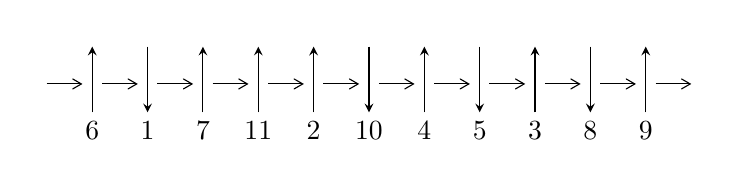
\begin{tikzpicture}[x=20pt, y=17pt]
	% nodes
	\node (C0) at (0, 0) {};
	\node (C1) at (1, 0) {};
	\node (C1U) at (1, +1) {};
	\node (C1D) at (1, -1) {6};

	\node (C2) at (2, 0) {};
	\node (C2U) at (2, +1) {};
	\node (C2D) at (2, -1) {1};

	\node (C3) at (3, 0) {};
	\node (C3U) at (3, +1) {};
	\node (C3D) at (3, -1) {7};

	\node (C4) at (4, 0) {};
	\node (C4U) at (4, +1) {};
	\node (C4D) at (4, -1) {11};

	\node (C5) at (5, 0) {};
	\node (C5U) at (5, +1) {};
	\node (C5D) at (5, -1) {2};

	\node (C6) at (6, 0) {};
	\node (C6U) at (6, +1) {};
	\node (C6D) at (6, -1) {10};

	\node (C7) at (7, 0) {};
	\node (C7U) at (7, +1) {};
	\node (C7D) at (7, -1) {4};

	\node (C8) at (8, 0) {};
	\node (C8U) at (8, +1) {};
	\node (C8D) at (8, -1) {5};

	\node (C9) at (9, 0) {};
	\node (C9U) at (9, +1) {};
	\node (C9D) at (9, -1) {3};

	\node (C10) at (10, 0) {};
	\node (C10U) at (10, +1) {};
	\node (C10D) at (10, -1) {8};

	\node (C11) at (11, 0) {};
	\node (C11U) at (11, +1) {};
	\node (C11D) at (11, -1) {9};
	\node (C12) at (12, 0) {};

	% arrows
	\draw[->,>={angle 60}]
	(C0) edge (C1) (C1) edge (C2) (C2) edge (C3) (C3) edge (C4) (C4) edge (C5) (C5) edge (C6) (C6) edge (C7) (C7) edge (C8) (C8) edge (C9) (C9) edge (C10) (C10) edge (C11) (C11) edge (C12) ;	\draw[->,>=stealth]
	(C1D) edge (C1U) (C2U) edge (C2D) (C3D) edge (C3U) (C4D) edge (C4U) (C5D) edge (C5U) (C6U) edge (C6D) (C7D) edge (C7U) (C8U) edge (C8D) (C9D) edge (C9U) (C10U) edge (C10D) (C11D) edge (C11U) ;
	\end{tikzpicture} \\
\hhline{~~} \\& 
\textbf{Solving Sequence} \\ \cline{2-2} 
 &
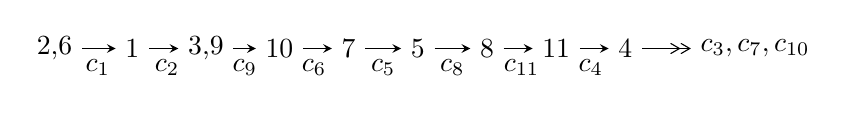
\begin{tikzpicture}[x=25pt, y=7pt]
	% node
	\node (A0) at (-1/8, 0) {2,6};
	\node (A1) at (1, 0) {1};
	\node (A2) at (33/16, 0) {3,9};
	\node (A3) at (25/8, 0) {10};
	\node (A4) at (33/8, 0) {7};
	\node (A5) at (41/8, 0) {5};
	\node (A6) at (49/8, 0) {8};
	\node (A7) at (57/8, 0) {11};
	\node (A8) at (65/8, 0) {4};
	\node (C1) at (1/2, -1) {$c_{1}$};
	\node (C2) at (3/2, -1) {$c_{2}$};
	\node (C3) at (21/8, -1) {$c_{9}$};
	\node (C4) at (29/8, -1) {$c_{6}$};
	\node (C5) at (37/8, -1) {$c_{5}$};
	\node (C6) at (45/8, -1) {$c_{8}$};
	\node (C7) at (53/8, -1) {$c_{11}$};
	\node (C8) at (61/8, -1) {$c_{4}$};
	\node (A9) at (10, 0) {$c_{3},c_{7},c_{10}$};

	% edge
	\draw[->,>=stealth]	
	(A0) edge (A1) (A1) edge (A2) (A2) edge (A3) (A3) edge (A4) (A4) edge (A5) (A5) edge (A6) (A6) edge (A7) (A7) edge (A8) ;
	\draw[->>,>={angle 60}]	
	(A8) edge (A9);
\end{tikzpicture} \\ 

\end{tabular} \\

\footnotetext{
The image of knot diagram is generated by the software ``\textbf{Draw programme}" developed by Andrew Bartholomew(\url{http://www.layer8.co.uk/maths/draw/index.htm\#Running-draw}), where we modified some parts for our purpose(\url{https://github.com/CATsTAILs/LinksPainter}).
}\phantom \\ \newline 
\centering \textbf{Ideals for irreducible components\footnotemark of $X_{\text{par}}$} 
 
\begin{align*}
I^u_{1}&=\langle 
-4.14827\times10^{147} u^{101}-7.64747\times10^{147} u^{100}+\cdots+1.69798\times10^{147} b+5.75046\times10^{144},\\
\phantom{I^u_{1}}&\phantom{= \langle  }-2.00222\times10^{146} u^{101}-2.26353\times10^{146} u^{100}+\cdots+1.69798\times10^{147} a+8.74321\times10^{147},\\
\phantom{I^u_{1}}&\phantom{= \langle  }u^{102}+2 u^{101}+\cdots+5 u-1\rangle \\
I^u_{2}&=\langle 
4 u^{18}+3 u^{17}+\cdots+b-5,\;-4 u^{18}-6 u^{17}+\cdots+a+3,\;u^{19}+u^{18}+\cdots+3 u+1\rangle \\
\\
\end{align*}
\raggedright * 2 irreducible components of $\dim_{\mathbb{C}}=0$, with total 121 representations.\\
\footnotetext{All coefficients of polynomials are rational numbers. But the coefficients are sometimes approximated in decimal forms when there is not enough margin.}
\newpage
\renewcommand{\arraystretch}{1}
\centering \section*{I. $I^u_{1}= \langle -4.15\times10^{147} u^{101}-7.65\times10^{147} u^{100}+\cdots+1.70\times10^{147} b+5.75\times10^{144},\;-2.00\times10^{146} u^{101}-2.26\times10^{146} u^{100}+\cdots+1.70\times10^{147} a+8.74\times10^{147},\;u^{102}+2 u^{101}+\cdots+5 u-1 \rangle$}
\flushleft \textbf{(i) Arc colorings}\\
\begin{tabular}{m{7pt} m{180pt} m{7pt} m{180pt} }
\flushright $a_{2}=$&$\begin{pmatrix}1\\0\end{pmatrix}$ \\
\flushright $a_{6}=$&$\begin{pmatrix}0\\u\end{pmatrix}$ \\
\flushright $a_{1}=$&$\begin{pmatrix}1\\u^2\end{pmatrix}$ \\
\flushright $a_{3}=$&$\begin{pmatrix}u^2+1\\u^4\end{pmatrix}$ \\
\flushright $a_{9}=$&$\begin{pmatrix}0.117918 u^{101}+0.133307 u^{100}+\cdots+12.2631 u-5.14920\\2.44307 u^{101}+4.50387 u^{100}+\cdots-4.24920 u-0.00338666\end{pmatrix}$ \\
\flushright $a_{10}=$&$\begin{pmatrix}-1.05197 u^{101}-1.12612 u^{100}+\cdots+5.29937 u-4.08217\\4.90798 u^{101}+8.02139 u^{100}+\cdots-3.48445 u-0.513579\end{pmatrix}$ \\
\flushright $a_{7}=$&$\begin{pmatrix}1.14572 u^{101}+2.76876 u^{100}+\cdots-11.5438 u-3.13970\\-0.725552 u^{101}-2.61060 u^{100}+\cdots-13.1281 u+3.50792\end{pmatrix}$ \\
\flushright $a_{5}=$&$\begin{pmatrix}- u\\u\end{pmatrix}$ \\
\flushright $a_{8}=$&$\begin{pmatrix}-1.79267 u^{101}-1.47114 u^{100}+\cdots+17.2481 u-5.63399\\4.35366 u^{101}+6.10832 u^{100}+\cdots-9.23414 u+0.481405\end{pmatrix}$ \\
\flushright $a_{11}=$&$\begin{pmatrix}-0.708680 u^{101}-1.92696 u^{100}+\cdots+32.4688 u-0.824193\\-0.871481 u^{101}-1.34105 u^{100}+\cdots-1.53831 u-0.889909\end{pmatrix}$ \\
\flushright $a_{4}=$&$\begin{pmatrix}-4.67359 u^{101}-7.60736 u^{100}+\cdots+9.22531 u+6.10870\\3.83528 u^{101}+4.33379 u^{100}+\cdots+3.88585 u-2.23360\end{pmatrix}$\\ \flushright $a_{4}=$&$\begin{pmatrix}-4.67359 u^{101}-7.60736 u^{100}+\cdots+9.22531 u+6.10870\\3.83528 u^{101}+4.33379 u^{100}+\cdots+3.88585 u-2.23360\end{pmatrix}$\\&\end{tabular}
\flushleft \textbf{(ii) Obstruction class $= -1$}\\~\\
\flushleft \textbf{(iii) Cusp Shapes $= 1.09737 u^{101}-1.38542 u^{100}+\cdots+37.0844 u+1.81533$}\\~\\
\newpage\renewcommand{\arraystretch}{1}
\flushleft \textbf{(iv) u-Polynomials at the component}\newline \\
\begin{tabular}{m{50pt}|m{274pt}}
Crossings & \hspace{64pt}u-Polynomials at each crossing \\
\hline $$\begin{aligned}c_{1},c_{5}\end{aligned}$$&$\begin{aligned}
&u^{102}-2 u^{101}+\cdots-5 u-1
\end{aligned}$\\
\hline $$\begin{aligned}c_{2}\end{aligned}$$&$\begin{aligned}
&u^{102}+46 u^{101}+\cdots+37 u+1
\end{aligned}$\\
\hline $$\begin{aligned}c_{3},c_{7}\end{aligned}$$&$\begin{aligned}
&u^{102}-39 u^{100}+\cdots-21 u+1
\end{aligned}$\\
\hline $$\begin{aligned}c_{4}\end{aligned}$$&$\begin{aligned}
&u^{102}-2 u^{101}+\cdots+9118 u-2449
\end{aligned}$\\
\hline $$\begin{aligned}c_{6}\end{aligned}$$&$\begin{aligned}
&u^{102}-2 u^{101}+\cdots-326 u-71
\end{aligned}$\\
\hline $$\begin{aligned}c_{8}\end{aligned}$$&$\begin{aligned}
&u^{102}+3 u^{101}+\cdots-81 u-19
\end{aligned}$\\
\hline $$\begin{aligned}c_{9}\end{aligned}$$&$\begin{aligned}
&u^{102}-14 u^{100}+\cdots+64416 u+8677
\end{aligned}$\\
\hline $$\begin{aligned}c_{10}\end{aligned}$$&$\begin{aligned}
&u^{102}+3 u^{101}+\cdots+153 u-7
\end{aligned}$\\
\hline $$\begin{aligned}c_{11}\end{aligned}$$&$\begin{aligned}
&u^{102}-8 u^{101}+\cdots-17631 u+2935
\end{aligned}$\\
\hline
\end{tabular}\\~\\
\newpage\renewcommand{\arraystretch}{1}
\flushleft \textbf{(v) Riley Polynomials at the component}\newline \\
\begin{tabular}{m{50pt}|m{274pt}}
Crossings & \hspace{64pt}Riley Polynomials at each crossing \\
\hline $$\begin{aligned}c_{1},c_{5}\end{aligned}$$&$\begin{aligned}
&y^{102}+46 y^{101}+\cdots+37 y+1
\end{aligned}$\\
\hline $$\begin{aligned}c_{2}\end{aligned}$$&$\begin{aligned}
&y^{102}+26 y^{101}+\cdots-171 y+1
\end{aligned}$\\
\hline $$\begin{aligned}c_{3},c_{7}\end{aligned}$$&$\begin{aligned}
&y^{102}-78 y^{101}+\cdots+71 y+1
\end{aligned}$\\
\hline $$\begin{aligned}c_{4}\end{aligned}$$&$\begin{aligned}
&y^{102}-24 y^{101}+\cdots-245491930 y+5997601
\end{aligned}$\\
\hline $$\begin{aligned}c_{6}\end{aligned}$$&$\begin{aligned}
&y^{102}+16 y^{101}+\cdots+36292 y+5041
\end{aligned}$\\
\hline $$\begin{aligned}c_{8}\end{aligned}$$&$\begin{aligned}
&y^{102}-13 y^{101}+\cdots-22977 y+361
\end{aligned}$\\
\hline $$\begin{aligned}c_{9}\end{aligned}$$&$\begin{aligned}
&y^{102}-28 y^{101}+\cdots-473410006 y+75290329
\end{aligned}$\\
\hline $$\begin{aligned}c_{10}\end{aligned}$$&$\begin{aligned}
&y^{102}+13 y^{101}+\cdots-645 y+49
\end{aligned}$\\
\hline $$\begin{aligned}c_{11}\end{aligned}$$&$\begin{aligned}
&y^{102}-18 y^{101}+\cdots+127701409 y+8614225
\end{aligned}$\\
\hline
\end{tabular}\\~\\
\newpage\flushleft \textbf{(vi) Complex Volumes and Cusp Shapes}
$$\begin{array}{c|c|c}  
\text{Solutions to }I^u_{1}& \I (\text{vol} + \sqrt{-1}CS) & \text{Cusp shape}\\
 \hline 
\begin{aligned}
u &= \phantom{-}0.546716 + 0.841027 I \\
a &= -1.19778 + 1.67154 I \\
b &= \phantom{-}0.181876 - 1.221980 I\end{aligned}
 & \phantom{-}5.02215 + 2.31431 I & \phantom{-0.000000 } 0 \\ \hline\begin{aligned}
u &= \phantom{-}0.546716 - 0.841027 I \\
a &= -1.19778 - 1.67154 I \\
b &= \phantom{-}0.181876 + 1.221980 I\end{aligned}
 & \phantom{-}5.02215 - 2.31431 I & \phantom{-0.000000 } 0 \\ \hline\begin{aligned}
u &= -0.910994 + 0.431263 I \\
a &= \phantom{-}1.33540 + 0.86176 I \\
b &= \phantom{-}0.152736 - 1.327330 I\end{aligned}
 & \phantom{-}6.30779 + 12.49790 I & \phantom{-0.000000 } 0 \\ \hline\begin{aligned}
u &= -0.910994 - 0.431263 I \\
a &= \phantom{-}1.33540 - 0.86176 I \\
b &= \phantom{-}0.152736 + 1.327330 I\end{aligned}
 & \phantom{-}6.30779 - 12.49790 I & \phantom{-0.000000 } 0 \\ \hline\begin{aligned}
u &= \phantom{-}0.913597 + 0.430094 I \\
a &= \phantom{-}1.30200 - 0.68866 I \\
b &= \phantom{-}0.205987 + 1.215020 I\end{aligned}
 & \phantom{-}1.31002 - 6.75104 I & \phantom{-0.000000 } 0 \\ \hline\begin{aligned}
u &= \phantom{-}0.913597 - 0.430094 I \\
a &= \phantom{-}1.30200 + 0.68866 I \\
b &= \phantom{-}0.205987 - 1.215020 I\end{aligned}
 & \phantom{-}1.31002 + 6.75104 I & \phantom{-0.000000 } 0 \\ \hline\begin{aligned}
u &= \phantom{-}0.518131 + 0.866736 I \\
a &= -1.32102 + 0.75450 I \\
b &= \phantom{-}1.63015 - 1.94328 I\end{aligned}
 & \phantom{-}4.96667 + 1.96860 I & \phantom{-0.000000 } 0 \\ \hline\begin{aligned}
u &= \phantom{-}0.518131 - 0.866736 I \\
a &= -1.32102 - 0.75450 I \\
b &= \phantom{-}1.63015 + 1.94328 I\end{aligned}
 & \phantom{-}4.96667 - 1.96860 I & \phantom{-0.000000 } 0 \\ \hline\begin{aligned}
u &= -0.936988 + 0.299819 I \\
a &= \phantom{-}1.62091 + 0.34671 I \\
b &= \phantom{-}0.232284 - 0.722761 I\end{aligned}
 & \phantom{-}5.22245 - 0.61170 I & \phantom{-0.000000 } 0 \\ \hline\begin{aligned}
u &= -0.936988 - 0.299819 I \\
a &= \phantom{-}1.62091 - 0.34671 I \\
b &= \phantom{-}0.232284 + 0.722761 I\end{aligned}
 & \phantom{-}5.22245 + 0.61170 I & \phantom{-0.000000 } 0\\
 \hline 
 \end{array}$$\newpage$$\begin{array}{c|c|c}  
\text{Solutions to }I^u_{1}& \I (\text{vol} + \sqrt{-1}CS) & \text{Cusp shape}\\
 \hline 
\begin{aligned}
u &= -0.348224 + 0.918489 I \\
a &= \phantom{-}0.068949 - 0.830583 I \\
b &= -0.452913 - 0.345870 I\end{aligned}
 & -1.76294 - 2.23528 I & \phantom{-0.000000 } 0 \\ \hline\begin{aligned}
u &= -0.348224 - 0.918489 I \\
a &= \phantom{-}0.068949 + 0.830583 I \\
b &= -0.452913 + 0.345870 I\end{aligned}
 & -1.76294 + 2.23528 I & \phantom{-0.000000 } 0 \\ \hline\begin{aligned}
u &= -0.424020 + 0.928079 I \\
a &= -0.042068 + 0.667634 I \\
b &= \phantom{-}1.140310 + 0.517906 I\end{aligned}
 & -2.05900 - 0.88708 I & \phantom{-0.000000 } 0 \\ \hline\begin{aligned}
u &= -0.424020 - 0.928079 I \\
a &= -0.042068 - 0.667634 I \\
b &= \phantom{-}1.140310 - 0.517906 I\end{aligned}
 & -2.05900 + 0.88708 I & \phantom{-0.000000 } 0 \\ \hline\begin{aligned}
u &= \phantom{-}0.768345 + 0.605608 I \\
a &= \phantom{-}1.130330 + 0.351165 I \\
b &= -0.99774 + 1.41995 I\end{aligned}
 & \phantom{-}7.07739 - 3.89935 I & \phantom{-0.000000 } 0 \\ \hline\begin{aligned}
u &= \phantom{-}0.768345 - 0.605608 I \\
a &= \phantom{-}1.130330 - 0.351165 I \\
b &= -0.99774 - 1.41995 I\end{aligned}
 & \phantom{-}7.07739 + 3.89935 I & \phantom{-0.000000 } 0 \\ \hline\begin{aligned}
u &= -0.161509 + 1.011950 I \\
a &= \phantom{-}1.237860 + 0.371151 I \\
b &= -0.396058 + 0.014652 I\end{aligned}
 & \phantom{-}1.72657 + 1.42609 I & \phantom{-0.000000 } 0 \\ \hline\begin{aligned}
u &= -0.161509 - 1.011950 I \\
a &= \phantom{-}1.237860 - 0.371151 I \\
b &= -0.396058 - 0.014652 I\end{aligned}
 & \phantom{-}1.72657 - 1.42609 I & \phantom{-0.000000 } 0 \\ \hline\begin{aligned}
u &= -0.762854 + 0.685546 I \\
a &= -0.77801 - 1.50504 I \\
b &= -0.21488 + 1.47469 I\end{aligned}
 & \phantom{-}5.99433 + 2.25625 I & \phantom{-0.000000 } 0 \\ \hline\begin{aligned}
u &= -0.762854 - 0.685546 I \\
a &= -0.77801 + 1.50504 I \\
b &= -0.21488 - 1.47469 I\end{aligned}
 & \phantom{-}5.99433 - 2.25625 I & \phantom{-0.000000 } 0\\
 \hline 
 \end{array}$$\newpage$$\begin{array}{c|c|c}  
\text{Solutions to }I^u_{1}& \I (\text{vol} + \sqrt{-1}CS) & \text{Cusp shape}\\
 \hline 
\begin{aligned}
u &= -0.381025 + 0.968579 I \\
a &= \phantom{-}2.32662 + 0.53559 I \\
b &= -2.41585 - 0.71894 I\end{aligned}
 & \phantom{-}0.30261 + 2.42814 I & \phantom{-0.000000 } 0 \\ \hline\begin{aligned}
u &= -0.381025 - 0.968579 I \\
a &= \phantom{-}2.32662 - 0.53559 I \\
b &= -2.41585 + 0.71894 I\end{aligned}
 & \phantom{-}0.30261 - 2.42814 I & \phantom{-0.000000 } 0 \\ \hline\begin{aligned}
u &= \phantom{-}0.380432 + 0.982651 I \\
a &= \phantom{-}1.51391 - 0.96311 I \\
b &= -1.62844 + 1.33790 I\end{aligned}
 & -3.75520 + 1.20274 I & \phantom{-0.000000 } 0 \\ \hline\begin{aligned}
u &= \phantom{-}0.380432 - 0.982651 I \\
a &= \phantom{-}1.51391 + 0.96311 I \\
b &= -1.62844 - 1.33790 I\end{aligned}
 & -3.75520 - 1.20274 I & \phantom{-0.000000 } 0 \\ \hline\begin{aligned}
u &= \phantom{-}0.907967 + 0.542230 I \\
a &= -0.358082 + 0.812397 I \\
b &= -0.233116 - 0.784920 I\end{aligned}
 & \phantom{-}3.25805 - 3.74660 I & \phantom{-0.000000 } 0 \\ \hline\begin{aligned}
u &= \phantom{-}0.907967 - 0.542230 I \\
a &= -0.358082 - 0.812397 I \\
b &= -0.233116 + 0.784920 I\end{aligned}
 & \phantom{-}3.25805 + 3.74660 I & \phantom{-0.000000 } 0 \\ \hline\begin{aligned}
u &= \phantom{-}0.336564 + 1.002720 I \\
a &= \phantom{-}0.793503 - 0.833640 I \\
b &= \phantom{-}0.354003 + 0.058896 I\end{aligned}
 & -0.65253 - 2.63980 I & \phantom{-0.000000 } 0 \\ \hline\begin{aligned}
u &= \phantom{-}0.336564 - 1.002720 I \\
a &= \phantom{-}0.793503 + 0.833640 I \\
b &= \phantom{-}0.354003 - 0.058896 I\end{aligned}
 & -0.65253 + 2.63980 I & \phantom{-0.000000 } 0 \\ \hline\begin{aligned}
u &= -0.867660 + 0.335592 I \\
a &= -0.547466 - 0.238777 I \\
b &= \phantom{-}0.267014 + 0.446348 I\end{aligned}
 & \phantom{-}1.38934 + 0.39182 I & \phantom{-0.000000 } 0 \\ \hline\begin{aligned}
u &= -0.867660 - 0.335592 I \\
a &= -0.547466 + 0.238777 I \\
b &= \phantom{-}0.267014 - 0.446348 I\end{aligned}
 & \phantom{-}1.38934 - 0.39182 I & \phantom{-0.000000 } 0\\
 \hline 
 \end{array}$$\newpage$$\begin{array}{c|c|c}  
\text{Solutions to }I^u_{1}& \I (\text{vol} + \sqrt{-1}CS) & \text{Cusp shape}\\
 \hline 
\begin{aligned}
u &= -0.838051 + 0.668944 I \\
a &= \phantom{-}1.075680 - 0.069757 I \\
b &= -0.646687 - 1.246750 I\end{aligned}
 & \phantom{-}2.82119 - 2.36401 I & \phantom{-0.000000 } 0 \\ \hline\begin{aligned}
u &= -0.838051 - 0.668944 I \\
a &= \phantom{-}1.075680 + 0.069757 I \\
b &= -0.646687 + 1.246750 I\end{aligned}
 & \phantom{-}2.82119 + 2.36401 I & \phantom{-0.000000 } 0 \\ \hline\begin{aligned}
u &= -0.504029 + 0.951532 I \\
a &= -2.24845 - 0.35174 I \\
b &= \phantom{-}1.96204 + 2.04629 I\end{aligned}
 & -1.51432 - 4.25684 I & \phantom{-0.000000 } 0 \\ \hline\begin{aligned}
u &= -0.504029 - 0.951532 I \\
a &= -2.24845 + 0.35174 I \\
b &= \phantom{-}1.96204 - 2.04629 I\end{aligned}
 & -1.51432 + 4.25684 I & \phantom{-0.000000 } 0 \\ \hline\begin{aligned}
u &= \phantom{-}0.886342 + 0.637949 I \\
a &= \phantom{-}0.939358 + 0.188412 I \\
b &= -0.867093 + 0.989781 I\end{aligned}
 & \phantom{-}7.56384 + 8.00259 I & \phantom{-0.000000 } 0 \\ \hline\begin{aligned}
u &= \phantom{-}0.886342 - 0.637949 I \\
a &= \phantom{-}0.939358 - 0.188412 I \\
b &= -0.867093 - 0.989781 I\end{aligned}
 & \phantom{-}7.56384 - 8.00259 I & \phantom{-0.000000 } 0 \\ \hline\begin{aligned}
u &= -0.505158 + 0.979164 I \\
a &= -1.39013 + 0.56499 I \\
b &= \phantom{-}1.10432 - 1.25247 I\end{aligned}
 & \phantom{-}1.08112 - 8.06609 I & \phantom{-0.000000 } 0 \\ \hline\begin{aligned}
u &= -0.505158 - 0.979164 I \\
a &= -1.39013 - 0.56499 I \\
b &= \phantom{-}1.10432 + 1.25247 I\end{aligned}
 & \phantom{-}1.08112 + 8.06609 I & \phantom{-0.000000 } 0 \\ \hline\begin{aligned}
u &= \phantom{-}0.711464 + 0.542127 I \\
a &= -1.09507 + 1.07155 I \\
b &= \phantom{-}0.116144 - 1.373020 I\end{aligned}
 & \phantom{-}2.68100 - 2.12226 I & \phantom{-0.000000 } 0 \\ \hline\begin{aligned}
u &= \phantom{-}0.711464 - 0.542127 I \\
a &= -1.09507 - 1.07155 I \\
b &= \phantom{-}0.116144 + 1.373020 I\end{aligned}
 & \phantom{-}2.68100 + 2.12226 I & \phantom{-0.000000 } 0\\
 \hline 
 \end{array}$$\newpage$$\begin{array}{c|c|c}  
\text{Solutions to }I^u_{1}& \I (\text{vol} + \sqrt{-1}CS) & \text{Cusp shape}\\
 \hline 
\begin{aligned}
u &= \phantom{-}0.472446 + 1.007140 I \\
a &= -0.498508 - 0.459792 I \\
b &= \phantom{-}0.226557 + 1.275670 I\end{aligned}
 & -3.15750 + 4.83334 I & \phantom{-0.000000 } 0 \\ \hline\begin{aligned}
u &= \phantom{-}0.472446 - 1.007140 I \\
a &= -0.498508 + 0.459792 I \\
b &= \phantom{-}0.226557 - 1.275670 I\end{aligned}
 & -3.15750 - 4.83334 I & \phantom{-0.000000 } 0 \\ \hline\begin{aligned}
u &= \phantom{-}0.512406 + 1.014650 I \\
a &= -2.28814 + 0.84392 I \\
b &= \phantom{-}1.63835 - 2.12595 I\end{aligned}
 & \phantom{-}0.47157 + 8.78333 I & \phantom{-0.000000 } 0 \\ \hline\begin{aligned}
u &= \phantom{-}0.512406 - 1.014650 I \\
a &= -2.28814 - 0.84392 I \\
b &= \phantom{-}1.63835 + 2.12595 I\end{aligned}
 & \phantom{-}0.47157 - 8.78333 I & \phantom{-0.000000 } 0 \\ \hline\begin{aligned}
u &= -0.443690 + 0.740067 I \\
a &= -1.47397 - 2.10514 I \\
b &= -0.38964 + 1.77473 I\end{aligned}
 & -0.768256 + 0.283969 I & \phantom{-0.000000 } 0 \\ \hline\begin{aligned}
u &= -0.443690 - 0.740067 I \\
a &= -1.47397 + 2.10514 I \\
b &= -0.38964 - 1.77473 I\end{aligned}
 & -0.768256 - 0.283969 I & \phantom{-0.000000 } 0 \\ \hline\begin{aligned}
u &= -0.485068 + 1.040750 I \\
a &= \phantom{-}1.083250 + 0.313226 I \\
b &= -0.96238 - 1.16637 I\end{aligned}
 & -0.62443 - 3.83028 I & \phantom{-0.000000 } 0 \\ \hline\begin{aligned}
u &= -0.485068 - 1.040750 I \\
a &= \phantom{-}1.083250 - 0.313226 I \\
b &= -0.96238 + 1.16637 I\end{aligned}
 & -0.62443 + 3.83028 I & \phantom{-0.000000 } 0 \\ \hline\begin{aligned}
u &= -0.714449 + 0.446789 I \\
a &= -1.39364 - 0.82917 I \\
b &= \phantom{-}0.49665 + 1.57085 I\end{aligned}
 & \phantom{-}6.25851 + 3.14258 I & \phantom{-}12.90912 - 3.40540 I \\ \hline\begin{aligned}
u &= -0.714449 - 0.446789 I \\
a &= -1.39364 + 0.82917 I \\
b &= \phantom{-}0.49665 - 1.57085 I\end{aligned}
 & \phantom{-}6.25851 - 3.14258 I & \phantom{-}12.90912 + 3.40540 I\\
 \hline 
 \end{array}$$\newpage$$\begin{array}{c|c|c}  
\text{Solutions to }I^u_{1}& \I (\text{vol} + \sqrt{-1}CS) & \text{Cusp shape}\\
 \hline 
\begin{aligned}
u &= -0.010623 + 1.160570 I \\
a &= \phantom{-}0.399937 - 0.342167 I \\
b &= -0.549931 - 0.398269 I\end{aligned}
 & -3.22104 - 2.07457 I & \phantom{-0.000000 } 0 \\ \hline\begin{aligned}
u &= -0.010623 - 1.160570 I \\
a &= \phantom{-}0.399937 + 0.342167 I \\
b &= -0.549931 + 0.398269 I\end{aligned}
 & -3.22104 + 2.07457 I & \phantom{-0.000000 } 0 \\ \hline\begin{aligned}
u &= \phantom{-}0.184970 + 0.814478 I \\
a &= \phantom{-}1.089970 - 0.393382 I \\
b &= -0.304161 - 0.600628 I\end{aligned}
 & -1.71950 - 1.55631 I & \phantom{-0.000000 -}0. + 5.16105 I \\ \hline\begin{aligned}
u &= \phantom{-}0.184970 - 0.814478 I \\
a &= \phantom{-}1.089970 + 0.393382 I \\
b &= -0.304161 + 0.600628 I\end{aligned}
 & -1.71950 + 1.55631 I & \phantom{-0.000000 } 0. - 5.16105 I \\ \hline\begin{aligned}
u &= -0.315832 + 1.121810 I \\
a &= \phantom{-}0.285651 + 1.088590 I \\
b &= -0.80567 - 1.77754 I\end{aligned}
 & \phantom{-}0.64011 - 4.17517 I & \phantom{-0.000000 } 0 \\ \hline\begin{aligned}
u &= -0.315832 - 1.121810 I \\
a &= \phantom{-}0.285651 - 1.088590 I \\
b &= -0.80567 + 1.77754 I\end{aligned}
 & \phantom{-}0.64011 + 4.17517 I & \phantom{-0.000000 } 0 \\ \hline\begin{aligned}
u &= \phantom{-}0.380666 + 1.110880 I \\
a &= \phantom{-}0.728299 + 0.343784 I \\
b &= -0.854582 + 0.712671 I\end{aligned}
 & -1.02724 + 3.84003 I & \phantom{-0.000000 } 0 \\ \hline\begin{aligned}
u &= \phantom{-}0.380666 - 1.110880 I \\
a &= \phantom{-}0.728299 - 0.343784 I \\
b &= -0.854582 - 0.712671 I\end{aligned}
 & -1.02724 - 3.84003 I & \phantom{-0.000000 } 0 \\ \hline\begin{aligned}
u &= -0.662917 + 0.979688 I \\
a &= -1.89971 - 0.56380 I \\
b &= \phantom{-}1.80912 + 1.53790 I\end{aligned}
 & \phantom{-}5.08526 - 7.66215 I & \phantom{-0.000000 } 0 \\ \hline\begin{aligned}
u &= -0.662917 - 0.979688 I \\
a &= -1.89971 + 0.56380 I \\
b &= \phantom{-}1.80912 - 1.53790 I\end{aligned}
 & \phantom{-}5.08526 + 7.66215 I & \phantom{-0.000000 } 0\\
 \hline 
 \end{array}$$\newpage$$\begin{array}{c|c|c}  
\text{Solutions to }I^u_{1}& \I (\text{vol} + \sqrt{-1}CS) & \text{Cusp shape}\\
 \hline 
\begin{aligned}
u &= -0.403141 + 0.700006 I \\
a &= \phantom{-}1.58780 - 0.55446 I \\
b &= -0.62884 + 1.29837 I\end{aligned}
 & \phantom{-}2.08822 + 4.14738 I & \phantom{-}5.91848 - 4.99016 I \\ \hline\begin{aligned}
u &= -0.403141 - 0.700006 I \\
a &= \phantom{-}1.58780 + 0.55446 I \\
b &= -0.62884 - 1.29837 I\end{aligned}
 & \phantom{-}2.08822 - 4.14738 I & \phantom{-}5.91848 + 4.99016 I \\ \hline\begin{aligned}
u &= -0.689076 + 0.977800 I \\
a &= \phantom{-}0.994641 + 0.951390 I \\
b &= \phantom{-}0.15446 - 1.53287 I\end{aligned}
 & \phantom{-}1.87918 - 3.30865 I & \phantom{-0.000000 } 0 \\ \hline\begin{aligned}
u &= -0.689076 - 0.977800 I \\
a &= \phantom{-}0.994641 - 0.951390 I \\
b &= \phantom{-}0.15446 + 1.53287 I\end{aligned}
 & \phantom{-}1.87918 + 3.30865 I & \phantom{-0.000000 } 0 \\ \hline\begin{aligned}
u &= \phantom{-}0.605344 + 1.038500 I \\
a &= -1.75704 + 0.85997 I \\
b &= \phantom{-}1.42964 - 1.72434 I\end{aligned}
 & \phantom{-}1.19886 + 7.18632 I & \phantom{-0.000000 } 0 \\ \hline\begin{aligned}
u &= \phantom{-}0.605344 - 1.038500 I \\
a &= -1.75704 - 0.85997 I \\
b &= \phantom{-}1.42964 + 1.72434 I\end{aligned}
 & \phantom{-}1.19886 - 7.18632 I & \phantom{-0.000000 } 0 \\ \hline\begin{aligned}
u &= \phantom{-}0.649296 + 1.019550 I \\
a &= \phantom{-}0.87338 - 1.39300 I \\
b &= \phantom{-}0.61169 + 1.58068 I\end{aligned}
 & \phantom{-}5.82598 + 9.26479 I & \phantom{-0.000000 } 0 \\ \hline\begin{aligned}
u &= \phantom{-}0.649296 - 1.019550 I \\
a &= \phantom{-}0.87338 + 1.39300 I \\
b &= \phantom{-}0.61169 - 1.58068 I\end{aligned}
 & \phantom{-}5.82598 - 9.26479 I & \phantom{-0.000000 } 0 \\ \hline\begin{aligned}
u &= \phantom{-}0.526098 + 1.098500 I \\
a &= -0.37261 + 1.45756 I \\
b &= \phantom{-}0.13000 - 1.71542 I\end{aligned}
 & \phantom{-}4.36168 + 3.54189 I & \phantom{-0.000000 } 0 \\ \hline\begin{aligned}
u &= \phantom{-}0.526098 - 1.098500 I \\
a &= -0.37261 - 1.45756 I \\
b &= \phantom{-}0.13000 + 1.71542 I\end{aligned}
 & \phantom{-}4.36168 - 3.54189 I & \phantom{-0.000000 } 0\\
 \hline 
 \end{array}$$\newpage$$\begin{array}{c|c|c}  
\text{Solutions to }I^u_{1}& \I (\text{vol} + \sqrt{-1}CS) & \text{Cusp shape}\\
 \hline 
\begin{aligned}
u &= \phantom{-}0.645470 + 0.436272 I \\
a &= -1.51263 - 0.10162 I \\
b &= \phantom{-}1.192850 - 0.631249 I\end{aligned}
 & \phantom{-}6.34669 + 1.05018 I & \phantom{-}13.33822 - 2.96795 I \\ \hline\begin{aligned}
u &= \phantom{-}0.645470 - 0.436272 I \\
a &= -1.51263 + 0.10162 I \\
b &= \phantom{-}1.192850 + 0.631249 I\end{aligned}
 & \phantom{-}6.34669 - 1.05018 I & \phantom{-}13.33822 + 2.96795 I \\ \hline\begin{aligned}
u &= \phantom{-}0.777412\phantom{ +0.000000I} \\
a &= \phantom{-}0.335267\phantom{ +0.000000I} \\
b &= \phantom{-}0.863939\phantom{ +0.000000I}\end{aligned}
 & \phantom{-}2.43364\phantom{ +0.000000I} & \phantom{-}3.98710\phantom{ +0.000000I} \\ \hline\begin{aligned}
u &= -0.586836 + 1.074450 I \\
a &= -1.74670 - 1.33399 I \\
b &= \phantom{-}1.16360 + 2.01117 I\end{aligned}
 & \phantom{-}4.41615 - 8.13681 I & \phantom{-0.000000 } 0 \\ \hline\begin{aligned}
u &= -0.586836 - 1.074450 I \\
a &= -1.74670 + 1.33399 I \\
b &= \phantom{-}1.16360 - 2.01117 I\end{aligned}
 & \phantom{-}4.41615 + 8.13681 I & \phantom{-0.000000 } 0 \\ \hline\begin{aligned}
u &= \phantom{-}0.754022 + 1.016080 I \\
a &= \phantom{-}0.531329 - 0.867731 I \\
b &= \phantom{-}0.341734 + 1.088120 I\end{aligned}
 & \phantom{-}6.42583 - 1.99123 I & \phantom{-0.000000 } 0 \\ \hline\begin{aligned}
u &= \phantom{-}0.754022 - 1.016080 I \\
a &= \phantom{-}0.531329 + 0.867731 I \\
b &= \phantom{-}0.341734 - 1.088120 I\end{aligned}
 & \phantom{-}6.42583 + 1.99123 I & \phantom{-0.000000 } 0 \\ \hline\begin{aligned}
u &= -0.077721 + 1.282840 I \\
a &= -0.350452 + 0.006592 I \\
b &= -0.345037 - 0.763343 I\end{aligned}
 & \phantom{-}0.16785 + 9.63948 I & \phantom{-0.000000 } 0 \\ \hline\begin{aligned}
u &= -0.077721 - 1.282840 I \\
a &= -0.350452 - 0.006592 I \\
b &= -0.345037 + 0.763343 I\end{aligned}
 & \phantom{-}0.16785 - 9.63948 I & \phantom{-0.000000 } 0 \\ \hline\begin{aligned}
u &= \phantom{-}0.685100 + 1.110090 I \\
a &= -1.239840 + 0.322500 I \\
b &= \phantom{-}1.24636 - 0.96116 I\end{aligned}
 & \phantom{-}1.48920 + 9.62261 I & \phantom{-0.000000 } 0\\
 \hline 
 \end{array}$$\newpage$$\begin{array}{c|c|c}  
\text{Solutions to }I^u_{1}& \I (\text{vol} + \sqrt{-1}CS) & \text{Cusp shape}\\
 \hline 
\begin{aligned}
u &= \phantom{-}0.685100 - 1.110090 I \\
a &= -1.239840 - 0.322500 I \\
b &= \phantom{-}1.24636 + 0.96116 I\end{aligned}
 & \phantom{-}1.48920 - 9.62261 I & \phantom{-0.000000 } 0 \\ \hline\begin{aligned}
u &= -0.623130 + 1.152470 I \\
a &= -0.816737 - 0.612012 I \\
b &= \phantom{-}0.731605 + 1.070220 I\end{aligned}
 & -1.01285 - 5.88545 I & \phantom{-0.000000 } 0 \\ \hline\begin{aligned}
u &= -0.623130 - 1.152470 I \\
a &= -0.816737 + 0.612012 I \\
b &= \phantom{-}0.731605 - 1.070220 I\end{aligned}
 & -1.01285 + 5.88545 I & \phantom{-0.000000 } 0 \\ \hline\begin{aligned}
u &= \phantom{-}0.070552 + 1.313550 I \\
a &= -0.0567565 - 0.0089612 I \\
b &= -0.590662 + 0.645402 I\end{aligned}
 & -4.91138 - 3.81366 I & \phantom{-0.000000 } 0 \\ \hline\begin{aligned}
u &= \phantom{-}0.070552 - 1.313550 I \\
a &= -0.0567565 + 0.0089612 I \\
b &= -0.590662 - 0.645402 I\end{aligned}
 & -4.91138 + 3.81366 I & \phantom{-0.000000 } 0 \\ \hline\begin{aligned}
u &= \phantom{-}0.656232 + 1.143470 I \\
a &= \phantom{-}1.47930 - 0.87156 I \\
b &= -1.26803 + 2.14541 I\end{aligned}
 & -0.85558 + 12.50630 I & \phantom{-0.000000 } 0 \\ \hline\begin{aligned}
u &= \phantom{-}0.656232 - 1.143470 I \\
a &= \phantom{-}1.47930 + 0.87156 I \\
b &= -1.26803 - 2.14541 I\end{aligned}
 & -0.85558 - 12.50630 I & \phantom{-0.000000 } 0 \\ \hline\begin{aligned}
u &= -0.654776 + 1.144510 I \\
a &= \phantom{-}1.59713 + 0.98601 I \\
b &= -1.38915 - 2.21983 I\end{aligned}
 & \phantom{-}4.1396 - 18.2450 I & \phantom{-0.000000 } 0 \\ \hline\begin{aligned}
u &= -0.654776 - 1.144510 I \\
a &= \phantom{-}1.59713 - 0.98601 I \\
b &= -1.38915 + 2.21983 I\end{aligned}
 & \phantom{-}4.1396 + 18.2450 I & \phantom{-0.000000 } 0 \\ \hline\begin{aligned}
u &= -0.613398 + 0.253704 I \\
a &= \phantom{-}0.726159 + 0.137434 I \\
b &= \phantom{-}0.348798 - 0.412040 I\end{aligned}
 & \phantom{-}1.49929 - 0.29141 I & \phantom{-}5.98153 + 0.11289 I\\
 \hline 
 \end{array}$$\newpage$$\begin{array}{c|c|c}  
\text{Solutions to }I^u_{1}& \I (\text{vol} + \sqrt{-1}CS) & \text{Cusp shape}\\
 \hline 
\begin{aligned}
u &= -0.613398 - 0.253704 I \\
a &= \phantom{-}0.726159 - 0.137434 I \\
b &= \phantom{-}0.348798 + 0.412040 I\end{aligned}
 & \phantom{-}1.49929 + 0.29141 I & \phantom{-}5.98153 - 0.11289 I \\ \hline\begin{aligned}
u &= -0.639970\phantom{ +0.000000I} \\
a &= \phantom{-}0.00425908\phantom{ +0.000000I} \\
b &= \phantom{-}0.486824\phantom{ +0.000000I}\end{aligned}
 & \phantom{-}1.15599\phantom{ +0.000000I} & \phantom{-}11.7830\phantom{ +0.000000I} \\ \hline\begin{aligned}
u &= \phantom{-}0.300150 + 0.557793 I \\
a &= -2.11925 + 1.68467 I \\
b &= \phantom{-}0.16460 - 1.80636 I\end{aligned}
 & \phantom{-}1.94932 - 4.82613 I & \phantom{-}5.93840 + 5.80122 I \\ \hline\begin{aligned}
u &= \phantom{-}0.300150 - 0.557793 I \\
a &= -2.11925 - 1.68467 I \\
b &= \phantom{-}0.16460 + 1.80636 I\end{aligned}
 & \phantom{-}1.94932 + 4.82613 I & \phantom{-}5.93840 - 5.80122 I \\ \hline\begin{aligned}
u &= -0.687034 + 1.194130 I \\
a &= \phantom{-}1.117490 + 0.759585 I \\
b &= -1.04280 - 2.27076 I\end{aligned}
 & \phantom{-}2.56452 - 5.34624 I & \phantom{-0.000000 } 0 \\ \hline\begin{aligned}
u &= -0.687034 - 1.194130 I \\
a &= \phantom{-}1.117490 - 0.759585 I \\
b &= -1.04280 + 2.27076 I\end{aligned}
 & \phantom{-}2.56452 + 5.34624 I & \phantom{-0.000000 } 0 \\ \hline\begin{aligned}
u &= -0.235498 + 1.372370 I \\
a &= \phantom{-}0.214681 - 0.146318 I \\
b &= -0.370603 + 0.393439 I\end{aligned}
 & -4.11255 - 3.30494 I & \phantom{-0.000000 } 0 \\ \hline\begin{aligned}
u &= -0.235498 - 1.372370 I \\
a &= \phantom{-}0.214681 + 0.146318 I \\
b &= -0.370603 - 0.393439 I\end{aligned}
 & -4.11255 + 3.30494 I & \phantom{-0.000000 } 0 \\ \hline\begin{aligned}
u &= \phantom{-}0.290031 + 0.120688 I \\
a &= \phantom{-}2.87656 + 0.87251 I \\
b &= -0.070464 - 0.476487 I\end{aligned}
 & -1.38492 - 1.35842 I & -0.44992 + 2.98076 I \\ \hline\begin{aligned}
u &= \phantom{-}0.290031 - 0.120688 I \\
a &= \phantom{-}2.87656 - 0.87251 I \\
b &= -0.070464 + 0.476487 I\end{aligned}
 & -1.38492 + 1.35842 I & -0.44992 - 2.98076 I\\
 \hline 
 \end{array}$$\newpage$$\begin{array}{c|c|c}  
\text{Solutions to }I^u_{1}& \I (\text{vol} + \sqrt{-1}CS) & \text{Cusp shape}\\
 \hline 
\begin{aligned}
u &= \phantom{-}0.072640 + 0.207452 I \\
a &= -4.59578 + 2.52040 I \\
b &= \phantom{-}0.216472 - 1.280150 I\end{aligned}
 & \phantom{-}1.92621 - 4.88869 I & \phantom{-}6.37356 + 5.88182 I \\ \hline\begin{aligned}
u &= \phantom{-}0.072640 - 0.207452 I \\
a &= -4.59578 - 2.52040 I \\
b &= \phantom{-}0.216472 + 1.280150 I\end{aligned}
 & \phantom{-}1.92621 + 4.88869 I & \phantom{-}6.37356 - 5.88182 I\\
 \hline 
 \end{array}$$\newpage\newpage\renewcommand{\arraystretch}{1}
\centering \section*{II. $I^u_{2}= \langle 4 u^{18}+3 u^{17}+\cdots+b-5,\;-4 u^{18}-6 u^{17}+\cdots+a+3,\;u^{19}+u^{18}+\cdots+3 u+1 \rangle$}
\flushleft \textbf{(i) Arc colorings}\\
\begin{tabular}{m{7pt} m{180pt} m{7pt} m{180pt} }
\flushright $a_{2}=$&$\begin{pmatrix}1\\0\end{pmatrix}$ \\
\flushright $a_{6}=$&$\begin{pmatrix}0\\u\end{pmatrix}$ \\
\flushright $a_{1}=$&$\begin{pmatrix}1\\u^2\end{pmatrix}$ \\
\flushright $a_{3}=$&$\begin{pmatrix}u^2+1\\u^4\end{pmatrix}$ \\
\flushright $a_{9}=$&$\begin{pmatrix}4 u^{18}+6 u^{17}+\cdots- u-3\\-4 u^{18}-3 u^{17}+\cdots+11 u+5\end{pmatrix}$ \\
\flushright $a_{10}=$&$\begin{pmatrix}3 u^{18}+5 u^{17}+\cdots- u-2\\-3 u^{18}-2 u^{17}+\cdots+11 u+5\end{pmatrix}$ \\
\flushright $a_{7}=$&$\begin{pmatrix}-4 u^{18}-5 u^{17}+\cdots+6 u+4\\6 u^{18}+10 u^{17}+\cdots+24 u^2+8 u\end{pmatrix}$ \\
\flushright $a_{5}=$&$\begin{pmatrix}- u\\u\end{pmatrix}$ \\
\flushright $a_{8}=$&$\begin{pmatrix}4 u^{18}+5 u^{17}+\cdots-10 u-6\\-4 u^{18}-2 u^{17}+\cdots+20 u+8\end{pmatrix}$ \\
\flushright $a_{11}=$&$\begin{pmatrix}-6 u^{18}-4 u^{17}+\cdots+12 u+3\\6 u^{18}+7 u^{17}+\cdots- u-1\end{pmatrix}$ \\
\flushright $a_{4}=$&$\begin{pmatrix}2 u^{18}+9 u^{16}+\cdots-3 u+1\\3 u^{18}+6 u^{17}+\cdots+21 u^2+8 u\end{pmatrix}$\\ \flushright $a_{4}=$&$\begin{pmatrix}2 u^{18}+9 u^{16}+\cdots-3 u+1\\3 u^{18}+6 u^{17}+\cdots+21 u^2+8 u\end{pmatrix}$\\&\end{tabular}
\flushleft \textbf{(ii) Obstruction class $= 1$}\\~\\
\flushleft \textbf{(iii) Cusp Shapes $= 9 u^{18}-7 u^{17}+21 u^{16}-64 u^{15}-7 u^{14}-180 u^{13}-111 u^{12}-308 u^{11}-298 u^{10}-355 u^9-411 u^8-322 u^7-405 u^6-284 u^5-267 u^4-199 u^3-123 u^2-75 u-18$}\\~\\
\newpage\renewcommand{\arraystretch}{1}
\flushleft \textbf{(iv) u-Polynomials at the component}\newline \\
\begin{tabular}{m{50pt}|m{274pt}}
Crossings & \hspace{64pt}u-Polynomials at each crossing \\
\hline $$\begin{aligned}c_{1}\end{aligned}$$&$\begin{aligned}
&u^{19}+u^{18}+\cdots+3 u+1
\end{aligned}$\\
\hline $$\begin{aligned}c_{2}\end{aligned}$$&$\begin{aligned}
&u^{19}+11 u^{18}+\cdots-3 u-1
\end{aligned}$\\
\hline $$\begin{aligned}c_{3}\end{aligned}$$&$\begin{aligned}
&u^{19}- u^{18}+\cdots+3 u+1
\end{aligned}$\\
\hline $$\begin{aligned}c_{4}\end{aligned}$$&$\begin{aligned}
&u^{19}+u^{18}+\cdots+4 u^2-1
\end{aligned}$\\
\hline $$\begin{aligned}c_{5}\end{aligned}$$&$\begin{aligned}
&u^{19}- u^{18}+\cdots+3 u-1
\end{aligned}$\\
\hline $$\begin{aligned}c_{6}\end{aligned}$$&$\begin{aligned}
&u^{19}+u^{18}+\cdots+2 u-1
\end{aligned}$\\
\hline $$\begin{aligned}c_{7}\end{aligned}$$&$\begin{aligned}
&u^{19}+u^{18}+\cdots+3 u-1
\end{aligned}$\\
\hline $$\begin{aligned}c_{8}\end{aligned}$$&$\begin{aligned}
&u^{19}-4 u^{17}+\cdots- u+1
\end{aligned}$\\
\hline $$\begin{aligned}c_{9}\end{aligned}$$&$\begin{aligned}
&u^{19}- u^{18}+\cdots-4 u+1
\end{aligned}$\\
\hline $$\begin{aligned}c_{10}\end{aligned}$$&$\begin{aligned}
&u^{19}+10 u^{18}+\cdots+u+1
\end{aligned}$\\
\hline $$\begin{aligned}c_{11}\end{aligned}$$&$\begin{aligned}
&u^{19}-9 u^{18}+\cdots+9 u-1
\end{aligned}$\\
\hline
\end{tabular}\\~\\
\newpage\renewcommand{\arraystretch}{1}
\flushleft \textbf{(v) Riley Polynomials at the component}\newline \\
\begin{tabular}{m{50pt}|m{274pt}}
Crossings & \hspace{64pt}Riley Polynomials at each crossing \\
\hline $$\begin{aligned}c_{1},c_{5}\end{aligned}$$&$\begin{aligned}
&y^{19}+11 y^{18}+\cdots-3 y-1
\end{aligned}$\\
\hline $$\begin{aligned}c_{2}\end{aligned}$$&$\begin{aligned}
&y^{19}- y^{18}+\cdots+y-1
\end{aligned}$\\
\hline $$\begin{aligned}c_{3},c_{7}\end{aligned}$$&$\begin{aligned}
&y^{19}-17 y^{18}+\cdots+11 y-1
\end{aligned}$\\
\hline $$\begin{aligned}c_{4}\end{aligned}$$&$\begin{aligned}
&y^{19}-3 y^{18}+\cdots+8 y-1
\end{aligned}$\\
\hline $$\begin{aligned}c_{6}\end{aligned}$$&$\begin{aligned}
&y^{19}+5 y^{18}+\cdots-2 y-1
\end{aligned}$\\
\hline $$\begin{aligned}c_{8}\end{aligned}$$&$\begin{aligned}
&y^{19}-8 y^{18}+\cdots+3 y-1
\end{aligned}$\\
\hline $$\begin{aligned}c_{9}\end{aligned}$$&$\begin{aligned}
&y^{19}+y^{18}+\cdots+16 y-1
\end{aligned}$\\
\hline $$\begin{aligned}c_{10}\end{aligned}$$&$\begin{aligned}
&y^{19}+6 y^{18}+\cdots+11 y-1
\end{aligned}$\\
\hline $$\begin{aligned}c_{11}\end{aligned}$$&$\begin{aligned}
&y^{19}+7 y^{18}+\cdots-3 y-1
\end{aligned}$\\
\hline
\end{tabular}\\~\\
\newpage\flushleft \textbf{(vi) Complex Volumes and Cusp Shapes}
$$\begin{array}{c|c|c}  
\text{Solutions to }I^u_{2}& \I (\text{vol} + \sqrt{-1}CS) & \text{Cusp shape}\\
 \hline 
\begin{aligned}
u &= \phantom{-}0.756785 + 0.627945 I \\
a &= -0.452433 + 0.973447 I \\
b &= -0.207776 - 1.275560 I\end{aligned}
 & \phantom{-}4.17315 - 3.45944 I & \phantom{-}9.43557 + 4.00641 I \\ \hline\begin{aligned}
u &= \phantom{-}0.756785 - 0.627945 I \\
a &= -0.452433 - 0.973447 I \\
b &= -0.207776 + 1.275560 I\end{aligned}
 & \phantom{-}4.17315 + 3.45944 I & \phantom{-}9.43557 - 4.00641 I \\ \hline\begin{aligned}
u &= \phantom{-}0.339623 + 0.919258 I \\
a &= \phantom{-}2.24756 - 0.52382 I \\
b &= -1.321130 + 0.107053 I\end{aligned}
 & \phantom{-}0.86544 - 3.34083 I & \phantom{-}3.34354 + 4.41577 I \\ \hline\begin{aligned}
u &= \phantom{-}0.339623 - 0.919258 I \\
a &= \phantom{-}2.24756 + 0.52382 I \\
b &= -1.321130 - 0.107053 I\end{aligned}
 & \phantom{-}0.86544 + 3.34083 I & \phantom{-}3.34354 - 4.41577 I \\ \hline\begin{aligned}
u &= \phantom{-}0.289824 + 0.910566 I \\
a &= -0.139626 - 1.198030 I \\
b &= \phantom{-}0.45271 + 2.08321 I\end{aligned}
 & \phantom{-}0.97791 + 5.98873 I & \phantom{-}3.06705 - 8.24706 I \\ \hline\begin{aligned}
u &= \phantom{-}0.289824 - 0.910566 I \\
a &= -0.139626 + 1.198030 I \\
b &= \phantom{-}0.45271 - 2.08321 I\end{aligned}
 & \phantom{-}0.97791 - 5.98873 I & \phantom{-}3.06705 + 8.24706 I \\ \hline\begin{aligned}
u &= -0.412083 + 1.018240 I \\
a &= \phantom{-}0.838502 - 0.039949 I \\
b &= -0.96015 - 1.15690 I\end{aligned}
 & -2.67947 - 3.32318 I & -4.16053 + 3.59653 I \\ \hline\begin{aligned}
u &= -0.412083 - 1.018240 I \\
a &= \phantom{-}0.838502 + 0.039949 I \\
b &= -0.96015 + 1.15690 I\end{aligned}
 & -2.67947 + 3.32318 I & -4.16053 - 3.59653 I \\ \hline\begin{aligned}
u &= -0.295559 + 0.809856 I \\
a &= \phantom{-}0.86554 + 1.47296 I \\
b &= \phantom{-}0.422703 - 0.430824 I\end{aligned}
 & -1.72030 + 0.39989 I & -1.68186 - 0.51618 I \\ \hline\begin{aligned}
u &= -0.295559 - 0.809856 I \\
a &= \phantom{-}0.86554 - 1.47296 I \\
b &= \phantom{-}0.422703 + 0.430824 I\end{aligned}
 & -1.72030 - 0.39989 I & -1.68186 + 0.51618 I\\
 \hline 
 \end{array}$$\newpage$$\begin{array}{c|c|c}  
\text{Solutions to }I^u_{2}& \I (\text{vol} + \sqrt{-1}CS) & \text{Cusp shape}\\
 \hline 
\begin{aligned}
u &= -0.849830\phantom{ +0.000000I} \\
a &= \phantom{-}0.195511\phantom{ +0.000000I} \\
b &= \phantom{-}0.504885\phantom{ +0.000000I}\end{aligned}
 & \phantom{-}0.655524\phantom{ +0.000000I} & -7.38950\phantom{ +0.000000I} \\ \hline\begin{aligned}
u &= \phantom{-}0.612447 + 1.019280 I \\
a &= -1.83602 + 0.52614 I \\
b &= \phantom{-}1.41766 - 1.16542 I\end{aligned}
 & \phantom{-}2.94345 + 8.65071 I & \phantom{-}5.93756 - 9.11510 I \\ \hline\begin{aligned}
u &= \phantom{-}0.612447 - 1.019280 I \\
a &= -1.83602 - 0.52614 I \\
b &= \phantom{-}1.41766 + 1.16542 I\end{aligned}
 & \phantom{-}2.94345 - 8.65071 I & \phantom{-}5.93756 + 9.11510 I \\ \hline\begin{aligned}
u &= -0.643913 + 1.140600 I \\
a &= -1.18488 - 0.86715 I \\
b &= \phantom{-}1.04791 + 2.13371 I\end{aligned}
 & \phantom{-}2.40281 - 5.12847 I & \phantom{-}0.682236 - 1.181576 I \\ \hline\begin{aligned}
u &= -0.643913 - 1.140600 I \\
a &= -1.18488 + 0.86715 I \\
b &= \phantom{-}1.04791 - 2.13371 I\end{aligned}
 & \phantom{-}2.40281 + 5.12847 I & \phantom{-}0.682236 + 1.181576 I \\ \hline\begin{aligned}
u &= -0.185848 + 1.360350 I \\
a &= \phantom{-}0.0181661 + 0.0703459 I \\
b &= \phantom{-}0.260654 - 0.457432 I\end{aligned}
 & -4.05934 - 3.53517 I & \phantom{-}6.8503 + 17.2063 I \\ \hline\begin{aligned}
u &= -0.185848 - 1.360350 I \\
a &= \phantom{-}0.0181661 - 0.0703459 I \\
b &= \phantom{-}0.260654 + 0.457432 I\end{aligned}
 & -4.05934 + 3.53517 I & \phantom{-}6.8503 - 17.2063 I \\ \hline\begin{aligned}
u &= -0.536362 + 0.225069 I \\
a &= -2.45456 - 0.82764 I \\
b &= \phantom{-}0.634975 + 0.421993 I\end{aligned}
 & \phantom{-}4.99327 - 0.03621 I & \phantom{-}8.72091 - 1.39804 I \\ \hline\begin{aligned}
u &= -0.536362 - 0.225069 I \\
a &= -2.45456 + 0.82764 I \\
b &= \phantom{-}0.634975 - 0.421993 I\end{aligned}
 & \phantom{-}4.99327 + 0.03621 I & \phantom{-}8.72091 + 1.39804 I\\
 \hline 
 \end{array}$$\newpage
\newpage\renewcommand{\arraystretch}{1}
\centering \section*{ III. u-Polynomials}
\begin{tabular}{m{50pt}|m{274pt}}
Crossings & \hspace{64pt}u-Polynomials at each crossing \\
\hline $$\begin{aligned}c_{1}\end{aligned}$$&$\begin{aligned}
&(u^{19}+u^{18}+\cdots+3 u+1)(u^{102}-2 u^{101}+\cdots-5 u-1)
\end{aligned}$\\
\hline $$\begin{aligned}c_{2}\end{aligned}$$&$\begin{aligned}
&(u^{19}+11 u^{18}+\cdots-3 u-1)(u^{102}+46 u^{101}+\cdots+37 u+1)
\end{aligned}$\\
\hline $$\begin{aligned}c_{3}\end{aligned}$$&$\begin{aligned}
&(u^{19}- u^{18}+\cdots+3 u+1)(u^{102}-39 u^{100}+\cdots-21 u+1)
\end{aligned}$\\
\hline $$\begin{aligned}c_{4}\end{aligned}$$&$\begin{aligned}
&(u^{19}+u^{18}+\cdots+4 u^2-1)(u^{102}-2 u^{101}+\cdots+9118 u-2449)
\end{aligned}$\\
\hline $$\begin{aligned}c_{5}\end{aligned}$$&$\begin{aligned}
&(u^{19}- u^{18}+\cdots+3 u-1)(u^{102}-2 u^{101}+\cdots-5 u-1)
\end{aligned}$\\
\hline $$\begin{aligned}c_{6}\end{aligned}$$&$\begin{aligned}
&(u^{19}+u^{18}+\cdots+2 u-1)(u^{102}-2 u^{101}+\cdots-326 u-71)
\end{aligned}$\\
\hline $$\begin{aligned}c_{7}\end{aligned}$$&$\begin{aligned}
&(u^{19}+u^{18}+\cdots+3 u-1)(u^{102}-39 u^{100}+\cdots-21 u+1)
\end{aligned}$\\
\hline $$\begin{aligned}c_{8}\end{aligned}$$&$\begin{aligned}
&(u^{19}-4 u^{17}+\cdots- u+1)(u^{102}+3 u^{101}+\cdots-81 u-19)
\end{aligned}$\\
\hline $$\begin{aligned}c_{9}\end{aligned}$$&$\begin{aligned}
&(u^{19}- u^{18}+\cdots-4 u+1)(u^{102}-14 u^{100}+\cdots+64416 u+8677)
\end{aligned}$\\
\hline $$\begin{aligned}c_{10}\end{aligned}$$&$\begin{aligned}
&(u^{19}+10 u^{18}+\cdots+u+1)(u^{102}+3 u^{101}+\cdots+153 u-7)
\end{aligned}$\\
\hline $$\begin{aligned}c_{11}\end{aligned}$$&$\begin{aligned}
&(u^{19}-9 u^{18}+\cdots+9 u-1)(u^{102}-8 u^{101}+\cdots-17631 u+2935)
\end{aligned}$\\
\hline
\end{tabular}\newpage\renewcommand{\arraystretch}{1}
\centering \section*{ IV. Riley Polynomials}
\begin{tabular}{m{50pt}|m{274pt}}
Crossings & \hspace{64pt}Riley Polynomials at each crossing \\
\hline $$\begin{aligned}c_{1},c_{5}\end{aligned}$$&$\begin{aligned}
&(y^{19}+11 y^{18}+\cdots-3 y-1)(y^{102}+46 y^{101}+\cdots+37 y+1)
\end{aligned}$\\
\hline $$\begin{aligned}c_{2}\end{aligned}$$&$\begin{aligned}
&(y^{19}- y^{18}+\cdots+y-1)(y^{102}+26 y^{101}+\cdots-171 y+1)
\end{aligned}$\\
\hline $$\begin{aligned}c_{3},c_{7}\end{aligned}$$&$\begin{aligned}
&(y^{19}-17 y^{18}+\cdots+11 y-1)(y^{102}-78 y^{101}+\cdots+71 y+1)
\end{aligned}$\\
\hline $$\begin{aligned}c_{4}\end{aligned}$$&$\begin{aligned}
&(y^{19}-3 y^{18}+\cdots+8 y-1)\\
&\cdot(y^{102}-24 y^{101}+\cdots-245491930 y+5997601)
\end{aligned}$\\
\hline $$\begin{aligned}c_{6}\end{aligned}$$&$\begin{aligned}
&(y^{19}+5 y^{18}+\cdots-2 y-1)(y^{102}+16 y^{101}+\cdots+36292 y+5041)
\end{aligned}$\\
\hline $$\begin{aligned}c_{8}\end{aligned}$$&$\begin{aligned}
&(y^{19}-8 y^{18}+\cdots+3 y-1)(y^{102}-13 y^{101}+\cdots-22977 y+361)
\end{aligned}$\\
\hline $$\begin{aligned}c_{9}\end{aligned}$$&$\begin{aligned}
&(y^{19}+y^{18}+\cdots+16 y-1)\\
&\cdot(y^{102}-28 y^{101}+\cdots-473410006 y+75290329)
\end{aligned}$\\
\hline $$\begin{aligned}c_{10}\end{aligned}$$&$\begin{aligned}
&(y^{19}+6 y^{18}+\cdots+11 y-1)(y^{102}+13 y^{101}+\cdots-645 y+49)
\end{aligned}$\\
\hline $$\begin{aligned}c_{11}\end{aligned}$$&$\begin{aligned}
&(y^{19}+7 y^{18}+\cdots-3 y-1)\\
&\cdot(y^{102}-18 y^{101}+\cdots+127701409 y+8614225)
\end{aligned}$\\
\hline
\end{tabular}
\vskip 2pc
\end{document}